% ======================================================================
% col: 20

\chapter{Implementazione}
\label{chap:impl}
In questo capitolo verranno descritti i passaggi implementati per generare la raceline ottima data una
mappa.

Nel corso dello studio di questa tesi, è stato integrato un fork
\footnote{https://github.com/CL2-UWaterloo/Raceline-Optimization} della repository di
\cite{christ2021time}, utilizzandolo come base di partenza. In questa repository sono implementati gli
algoritmi analizzati al capitolo \ref{chap:opt} (pag.~\pageref{chap:opt}); quindi si è condotta
un'analisi del codice sorgente, identificando le parti rilevanti per lo scopo e apportando delle
modifiche e personalizzazioni per adattarlo al contesto, come per esempio selezionare i tipi di output da
produrre. Questo ha permesso di ottimizzare le funzionalità esistenti e di implementare ulteriori
miglioramenti, garantendo così che il codice rispondesse alle necessità dello studio.

\bigskip
\noindent I passaggi ad alto livello sono i seguenti:
\begin{enumerate}
	\item ottenere l'immagine di una mappa (per esempio attraverso \hyperref[par:slam]{SLAM});
	\item eventualmente ripulirla di imperfezioni e ottenere un circuito chiuso; 
	\item generare la centerline e calcolare la larghezza del circuito;
	\item applicare gli algoritmi di generazione della raceline;
\end{enumerate}
La mappa viene digitalizzata in file immagine che rappresenta una \textit{occupancy grid}, mentre i
percorsi, che siano raceline o centerline, sono in formato csv con due colonne rappresentanti la
posizione $(x,y)$ di ogni sample, nel caso sia una centerline, e una terza colonna per la velocità per
quanto riguarda la raceline ed eventualmente ulteriori colonne per altri valori come l'accelerazione e
l'angolo di sterzata.

Una occupancy grid è una immagine in scala di grigi in cui, per ogni pixel, viene rappresentata la
\textit{probabilità} che quel pixel sia uno spazio libero attraverso una percentuale di grigio. Dunque in
occupancy grid binarie, il nero indica l'ostacolo certo, mentre il bianco lo spazio libero.
\newpage
Di seguito si indicano le specifiche della macchina usata durante questa tesi:
\begin{itemize}
	\item[-] \textit{OS}: Ubuntu 22.04.4 LTS Jammy Jellyfish (kernel 6.8.0-45-generic)
	\item[-] \textit{Kernel}: 6.8.0-40 generic x86\_64
	\item[-] \textit{CPU}: Intel Core i7-6700k quad core
	\item[-] \textit{RAM}: 16GB
\end{itemize}

\section{Generazione centerline}
Affinché l'algoritmo per l'estrazione della linea di riferimento restituisca un risultato corretto
l'immagine della mappa deve rappresentare un circuito chiuso e con bordi ben
definiti e lisci, come effettivamente sarebbe un circuito di F1.
Dunque se si acquisisce una mappa con SLAM come in figura \ref{fig:slam_map} è necessario modificarla come
in figura \ref{fig:slam_map_mod}. Durante l'implementazione di questa tesi si è deciso di usare le mappe
dei circuiti da gara più famosi forniti da F1TENTH stesso \cite{f1tenth-gitmaps}.

\begin{figure}[H]
	\begin{minipage}[c]{0.47\textwidth}
		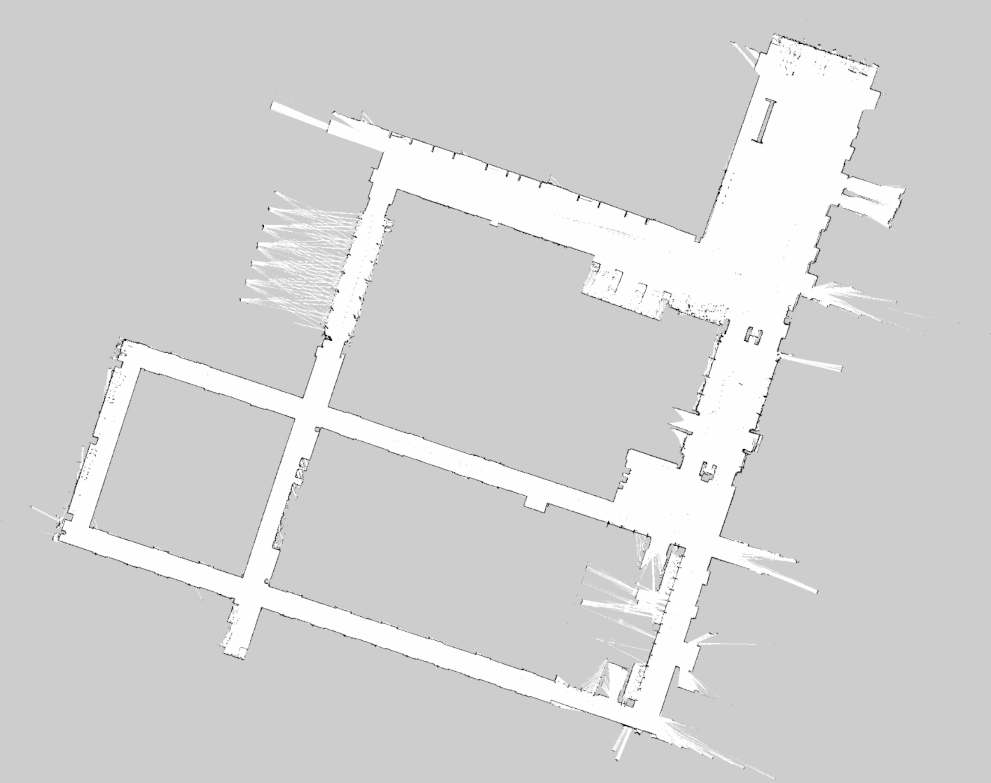
\includegraphics[width=1\textwidth]{slam_map.png}
		\caption{\raggedright Mappa risultante da SLAM \cite{stevengong} }
		\label{fig:slam_map}
	\end{minipage}\hfill
	\begin{minipage}[c]{0.47\textwidth}
		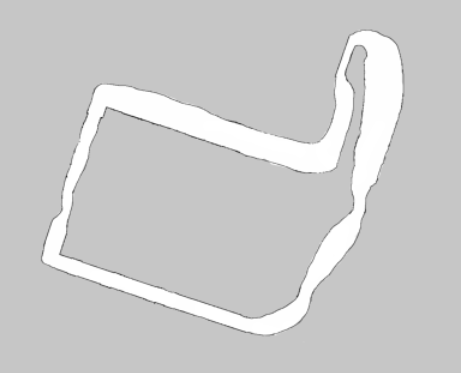
\includegraphics[width=1\textwidth]{slam_map_mod.png}
		\caption{Modifica dell'immagine~\ref{fig:slam_map} per creare un circuito chiuso \cite{stevengong} }
		\label{fig:slam_map_mod}
	\end{minipage}
\end{figure}

Operativamente, l'algoritmo usato per la generazione viene dal mondo dell'elaborazione delle immagini e
si chiama EDT (Euclidian Distance Transform), che calcola la distanza euclidea per ogni pixel
dell'immagine dal background: in questo caso, lo sfondo preso in considerazione sono i punti non
esplorati, ovvero quelli esterni ai bordi del circuito.
Un esempio di applicazione di EDT si trova all'immagine \ref{fig:edt-ex}.

\newgeometry{bottom=1cm}
Un aspetto da sottolineare è che le immagini fornite da F1TENTH rappresentano una occupancy grid
ternaria, in cui il grigio corrisponde alle zone non esplorate; per sfruttare l'algoritmo sopra citato è
necessario che i pixel grigi vengano convertiti in nero, perché è il valore considerato come background
dall'algoritmo EDT. Prendendo come riferimento il circuito di Monza all'immagine \ref{fig:monza-binary}, il
risultato dell'algoritmo si può vedere all'immagine \ref{fig:monza-edt}.
\begin{figure}[H]
	\begin{center}
		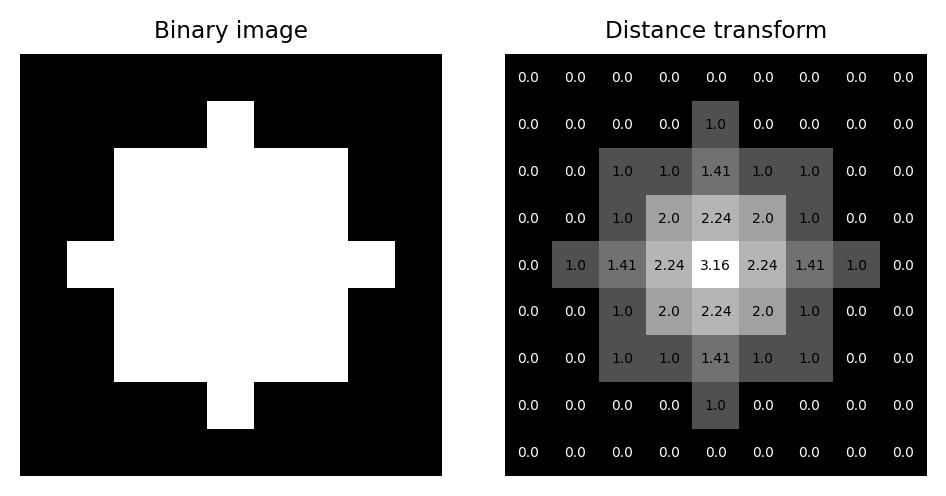
\includegraphics[width=1\textwidth]{edt-ex.png}
		\caption{Esempio di applicazione dell'algoritmo EDT su una immagine binaria, l'immagine a destra
		mostra il risultato indicando la distanza euclidea dal background per ogni pixel \cite{stevengong-edt} }
		\label{fig:edt-ex}
	\end{center}
\end{figure}
\begin{figure}[H]
	\begin{minipage}[c]{0.47\textwidth}
		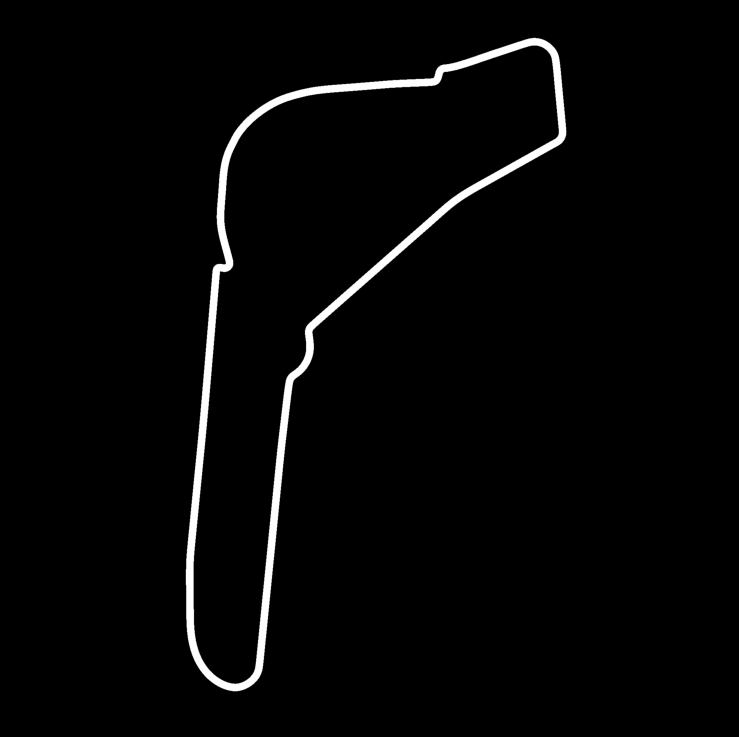
\includegraphics[width=1\textwidth]{monza-binary.png}
		\caption{Immagine della occupancy grid binaria del circuito di Monza}
		\label{fig:monza-binary}
	\end{minipage}\hfill
	\begin{minipage}[c]{0.47\textwidth}
		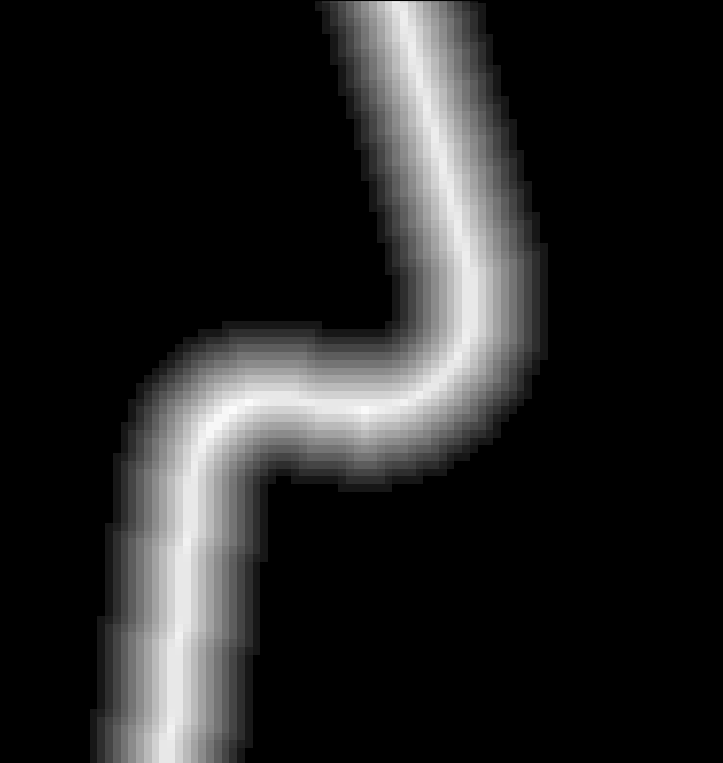
\includegraphics[width=1\textwidth]{monza-edt.png}
		\caption{\raggedright Risultato dell'algoritmo EDT mostrato sulla curva 1-2 del circuito di Monza}
		\label{fig:monza-edt}
	\end{minipage}
\end{figure}
\restoregeometry

Il passo successivo è quello di ottenere solo la parte centrale, ovvero quella con i valori di bianco
più alti e ridurla a un singolo pixel. In Python, questa operazione, viene eseguita dalla funzione
\verb|skeletonize()| del pacchetto \verb|scikit-image|. Seguendo l'esempio con il circuito di Monza, il
risultato di questa fase si può osservare all'immagine \ref{fig:monza-skel}.

A questo punto è necessario campionare il percorso di un pixel trovato: partendo da un punto del
percorso, si applica una ricerca DFS (Depth First Search) per trovare i successivi pixel bianchi. Dunque
da un pixel del percorso, si cerca il primo pixel bianco in tutte le direzioni che non sia già stato
esplorato: seguendo questo processo si ottengono le posizioni dei pixel e la loro distanza dai bordi, si
trasformano nel frame della mappa e esportano queste informazioni in un csv contenente le colonne
\verb|x, y, width_left, width_right|.
\vfill
\begin{figure}[H]
	\begin{center}
		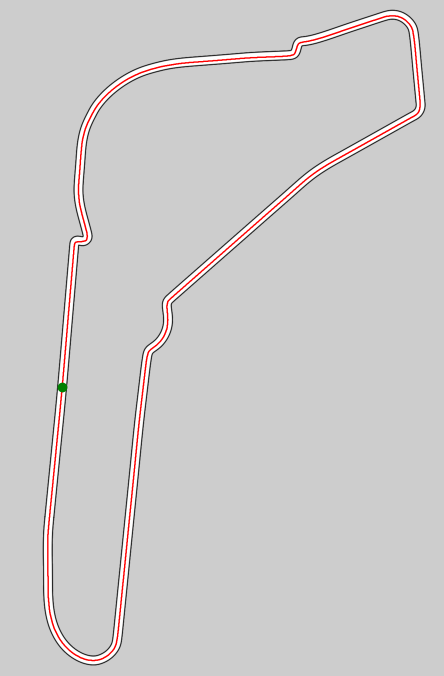
\includegraphics[width=0.6\textwidth, angle=90]{monza-skel.png}
	\end{center}
	\caption{Visualizzazione della centerline di Monza, il punto verde indica il punto di partenza}
	\label{fig:monza-skel}
\end{figure}

\newpage


\section{Esecuzione dell'ottimizzazione}
Ad alto livello, l'ottimizzazione cerca iterativamente di aggiustare la centerline in modo tale da
ottenere il risultato migliore, come spiegato nel capitolo~\ref{chap:opt} pag.~\pageref{chap:opt}.
Questa fase non richiede solamente di eseguire il programma solutore, ma è necessario
configurare i parametri che l'algoritmo usa. Questo compito si chiama \textit{tuning} dei parametri
e consiste nel trovare quelli che meglio si adattano nel trovare la soluzione migliore.

Durante lo studio di questa tesi il principale parametro modificato durante le prove è stato lo
\textit{stepsize}, ovvero la distanza, in metri, tra un sample e l'altro. In particolare si distinguono
tre stepsize diversi:
\begin{itemize}
	\item \verb|stepsize_prep|: viene usato per l'interpolazione lineare prima dell'approssimazione del
		percorso con la spline;
	\item \verb|stepsize_reg|: usato durante l'ottimizzazione per l'interpolazione della spline;
	\item \verb|stepsize_interp_after_opt|: usato per campionare la spline dopo l'ottimizzazione, è la
		distanza dei sample esportati nel csv risultante.
\end{itemize}
Altri parametri fanno riferimento alla dinamica del veicolo, come angolo di sterzata massimo e velocità
massima, e grandezze fisiche del veicolo, come massa, lunghezza e larghezza. Sono disponibili anche
parametri specifici per il tipo di ottimizzazione, per esempio un valore aggiuntivo alla larghezza del
veicolo che comprende un margine di sicurezza dai bordi del circuito. Di seguito si mostrano alcuni dei
valori usati che descrivono le proprietà del veicolo indipendentemente dal tipo di ottimizzazione usato:

\begin{lstlisting}
veh_params = {
	"v_max": 15.0,       # [m/s]
	"length": 0.58,      # [m]
	"width": 0.31,       # [m]
	"mass": 3.74,        # [Kg]
	"dragcoeff": 0.075,  # [kg*m^2/m^3]
	"curvlim": 3.0,      # [rad/m]
	"g": 9.81            # [N/Kg]
}
\end{lstlisting}
\newpage
\noindent Il risultato di questa fase è un file csv contenenti i samples della raceline generata. Di seguito si
mostra un esempio \footnote{per motivi di spazio si è scelto di mostrare solo 3 cifre decimali, durante
lo studio si è usata una precisione fino a 7 cifre dopo il punto} dei primi $6$ samples per il
file\\\texttt{mintime-28-09-2024\_18-12.csv} per il circuito di Spa:
\begin{lstlisting}
# s_m: distanza in metri della traiettoria
# x_m, y_m: posizione del sample nel frame della mappa
# psi_rad: orientamento del veicolo rispetto alla mappa
# kappa_radpm: curvatura per quel punto in rad/m
# vx_mps: velocita' in m/s
# ax_mps2: accelerazione in m/s^2

# s_m; x_m; y_m; psi_rad; kappa_radpm; vx_mps; ax_mps2
0.000,11.148,-65.899,-0.370,0.032,10.236,-1.072
0.149,11.202,-65.759,-0.365,0.032,10.220,-1.070
0.299,11.256,-65.618,-0.360,0.032,10.204,-1.068
0.449,11.308,-65.477,-0.355,0.032,10.189,-1.067
0.599,11.360,-65.336,-0.350,0.032,10.173,-1.065
0.749,11.412,-65.194,-0.345,0.032,10.157,-1.064
\end{lstlisting}
A fini di una migliore gestione, si è deciso di salvare il file di configurazione dei parametri e
l'output prodotto dallo script solutore e organizzarli in directory con data e ora dell'esecuzione; in
questo modo è stata facilitata la fase di tuning e la successiva analisi dei tracciati.

\begin{figure}[H]
	\begin{center}
		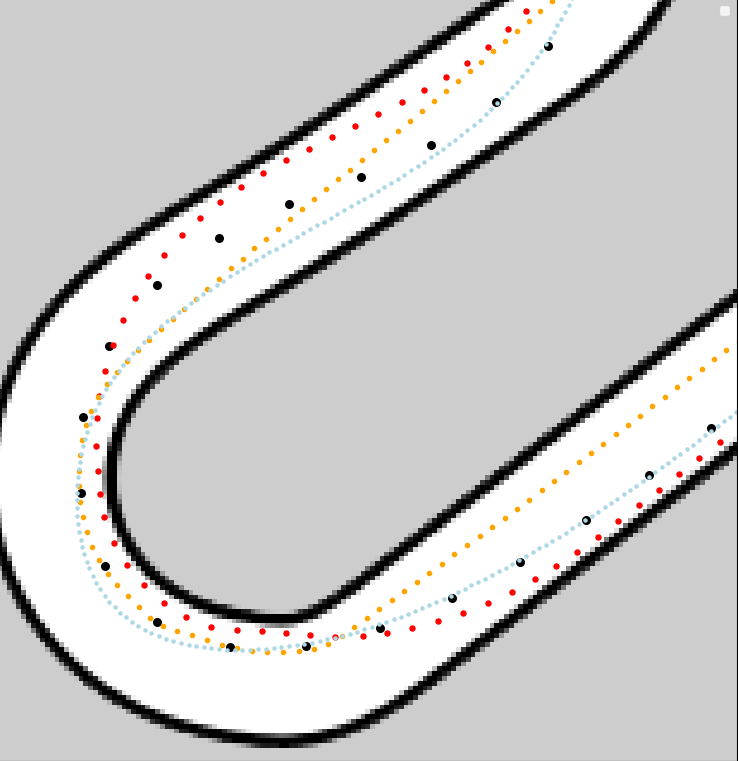
\includegraphics[width=0.72\textwidth]{stepsize.png}
	\end{center}
	\caption{Quattro traiettorie con stepsize diversi: nera a 1.5m, rossa a 0.5m,
	arancione a 0.3m e azzurra a 0.15m}
	\label{fig:stepsize}
\end{figure}

\subsection{Tuning dei parametri}
\label{par:tuning}
È facile immaginare che una minore distanza tra i sample durante l'ottimizzazione porti un risultato più
preciso a costo di aumentare il tempo di esecuzione, come è emerso nel capitolo
\href{sec:exec-time}{successivo} di analisi (pag.~\pageref{sec:exec-time}).
In figura~\ref{fig:stepsize} si visualizza una comparazione tra raceline con stepsize diversi.

Come ci si potrebbe aspettare, il parametro che controlla principalmente il tempo di esecuzione è lo
stepsize durante l'ottimizzazione, ovvero \verb|stepsize_reg|, per questo è stato necessario scegliere un
valore tale che bilanci bene la qualità del tracciato prodotto e il tempo di esecuzione. Infatti, per
evitare che l'ottimizzazione impieghi troppo tempo, il numero di iterazioni è limitato a 2000: se entro
questo limite non è stata trovata una soluzione viene ritornato un errore.

In linea generale, si è riscontrato che:
\begin{itemize}
	\item \verb|stepsize_prep|: per quanto riguarda il percorso più breve e la curvatura minima, impatta
		sulla qualità del risultato, diversamente dal tempo minimo; non influisce significativamente sul
		tempo di esecuzione. Valori in $[0.1, 0.5)$ per i primi due, $[0.5, 1]$ per mintime;
	\item \verb|stepsize_reg|: come accennato precedentemente, incide sul tempo di esecuzione
		e in modo apprezzabile per mintime; è significativo per la qualità del percorso. Valori $ > 0.3$
		per shortest path e mincurv, mentre per mintime sono necessari valori $> 1.0$ per evitare di
		sforare le 2000 iterazioni;
	\item \verb|stepsize_interp_after_opt|: non incide in modo sostanziale sul tempo e per questo può
		essere valorizzato in base alle necessità dell'algoritmo che userà il percorso.
\end{itemize}
A valori alti degli stepsize (es: $> 1.5$), può capitare che la raceline generata "tagli" il percorso per
curve molto rapide, come nella chicane di Spa. Questo è capitato principalmente con l'algoritmo del
percorso più breve, come mostrato alla figura \ref{fig:taglio-spa}

\begin{figure}[h]
	\begin{minipage}[c]{0.45\textwidth}
		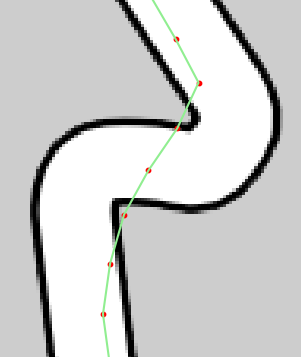
\includegraphics[width=0.3\textheight]{chicane_shpth.png}
		\caption{Generazione errata del percorso per via di stepsize troppo ampi}
		\label{fig:taglio-spa}
	\end{minipage}\hfill
	\begin{minipage}[c]{0.45\textwidth}
		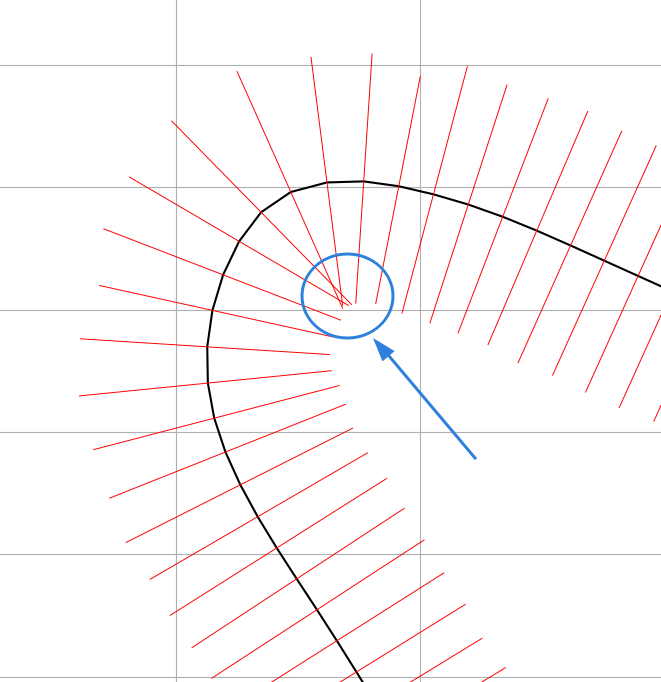
\includegraphics[width=\textwidth]{nomral-crossed.png}
		\caption{\raggedright Linee ortogonali alla centerline incrociate}
		\label{fig:norm-cross}
	\end{minipage}
\end{figure}
Altri parametri modificati durante le sperimentazioni sono qualità inerenti alle spline, principalmente
lo smoothing factor. Quest'ultimo, se troppo basso e in concomitanza con valori di stepsize bassi, può
generare delle linee ortogonali che si incrociano tra loro e che quindi non possono produrre un percorso
corretto. Un esempio di questo caso è visibile all'immagine \ref{fig:norm-cross}. Durante le
sperimentazioni questo valore è stato fissato a 80.
\noindent Di seguito si mostrano gli stepsize usati per generare il percorso a figura \ref{fig:taglio-spa}.
\begin{lstlisting}
stepsize_opts={
	"stepsize_prep": 1.0,
	"stepsize_reg": 1.5,
	"stepsize_interp_after_opt": 1.5
}
\end{lstlisting}
Mentre i successivi sono i parametri della spline e stepsize utilizzati per la figura \ref{fig:norm-cross}.

\begin{lstlisting}
stepsize_opts={
	"stepsize_prep": 0.1,
	"stepsize_reg": 0.5,
	"stepsize_interp_after_opt": 0.3
}

reg_smooth_opts={
	"k_reg": 3,   # grado della spline
	"s_reg": 1.0  # smoothing factor [1.0, 100]
}
\end{lstlisting}
